%%%
%% Design :: Use Case
%%%
\section{Use Case}
\label{sec:use_case}

A Use Case diagram illustrates ``a meaningful interaction with a computer 
system'', and provides various approaches to analysing system design 
requirements \citep{lunn03}. Within this section the use case of the entire 
proposed system will be presented and discussed. The use case has been split 
into two diagrams to increase the readability of the diagram.

The primary intended use of the system is to be able to submit a clue to be 
solved, which requires the clue, solution length and solution pattern. Figure 
\ref{fig:end_user_use_case} illustrates the three parameter requirements in 
order to submit a clue to be solved.

\begin{figure}[H]
  \centering
  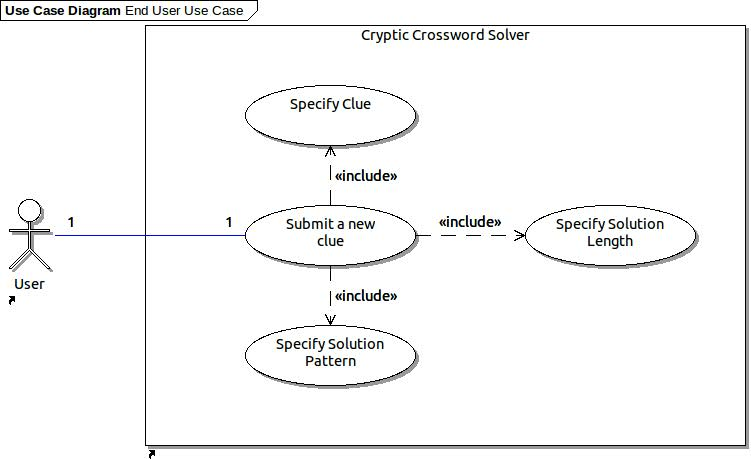
\includegraphics[width=0.9\textwidth]{use_case/end_user_use_case.jpg}
  \caption{Use case illustrating the actor's range of possibilities}
  \label{fig:end_user_use_case}
\end{figure}

It must be stated that the solution pattern could be unknown. In this instance a
set wild card characters must be given to the system. This was previously shown
in figure \ref{fig:input_activity} on page \pageref{fig:input_activity}. 

The remainder of the Use case is shown in figure \ref{fig:system_use_case}. Once
the user has input the various data elements the system will then attempt to 
solve the clue. 

\begin{figure}[H]
  \centering
  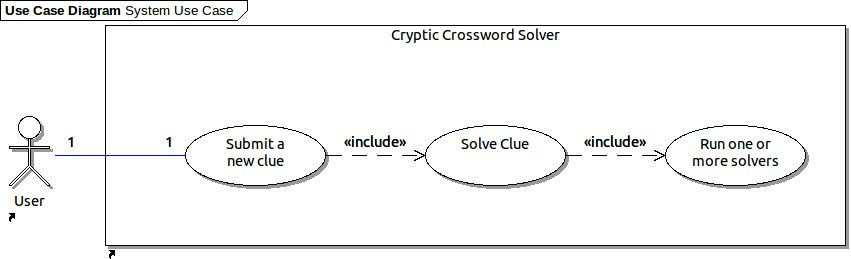
\includegraphics[width=0.9\textwidth]{use_case/system_use_case.jpg}
  \caption{System Use Case}
  \label{fig:system_use_case}
\end{figure}

The use case demonstrates that there is very little user input required, and 
once the data parameters have been entered there will be no additional user 
interaction required.

A design decision has been taken so that there is minimal user interaction with 
the service. This will be particularly useful for those who are using a mobile
device, as inputting data can be laborious in comparison to a desktop machine.
